\newpage
\section{Loss Functions and Optimization}
\subsection{Loss Functions}
Quantifies our unhappiness with the scores across the training data.

A loss function tells how good our current classifier is

Given a dataset of examples
\begin{align*}
    \{ (x_i, y_i) \}_{i=1}^N
\end{align*}
where $x_i$ is image and $y_i$ is (integer) label. 

Loss over the dataset is a sum of loss over examples:
\begin{align*}
    L=\frac{1}{N}\sum_i L_i (f(x_i, W), y_i)
\end{align*}

\subsubsection{Multiclass SVM loss}
Using the shorthand for the scores vector: $s=f(x_i, W)$. 

The SVM loss has the form:
\begin{align*}
    L_i&=\sum_{j\ne y_i}\left\{ \begin{array}{ll}
        0 & \text{if }s_{y_i}\le s_j+1\\
        s_j-s_{y_i}+1 & \text{otherwise}
    \end{array} \right.\\
    &=\sum_{j\ne y_i}\max(0, s_j-s_{y_i}+1)
\end{align*}
where $s_i$ is the $i$ label score.

此类型被成为``Hinge loss'' (铰链损失)

\begin{figure}[!htb]
    \centering
    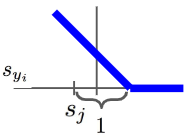
\includegraphics[width=0.309\textwidth]{pic/Lec3/SVM loss.png}
    \caption{SVM Loss}
\end{figure}

\textbf{Notes}:
\begin{enumerate}\small
    \item 在初始化$W$后的训练第一轮观察loss是否符合预期(这时的loss可计算一般), 帮助debug. 
    \item $L_i$ 中+1是调整了整个loss与$W$的比例, 其实并不重要, course note 上据说讨论了
    \item avg与sum也并不重要, 在这里只是调整了loss与$W$的比例
    \item 可以切换为非线性 loss
    \item 不同的loss考虑了不同的错误类型
\end{enumerate}

\subsubsection{Regularization}
\begin{align*}
    L(W)=\underbrace{\frac{1}{N}\sum_{i=1}^N L_i (f(x_i, W), y_i)}_{\text{Data loss}}+\underbrace{\lambda R(W)}_{\text{Regularization}}
\end{align*}
\begin{itemize}\small
    \item Data loss: Model predictions should match training data
    \item Regularization: Model should be ``simple'', so it works on test data
\end{itemize}

where $\lambda$  regularization strength (hyperparameter, 控制了二者权重). 

\begin{figure}[!htb]
    \centering
    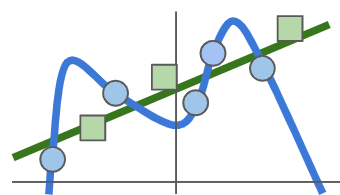
\includegraphics[width=0.309\textwidth]{pic/Lec3/Regularization.png}
    \caption{Blue is training data, Green is test data}
\end{figure}

``Among competing hypotheses, the simplest is the best''

\paragraph{In common use}:
\begin{itemize}\small
    \item L2 regularization $R(W)=\sum_k\sum_l W^2_{k,l}$ (鼓励$W$均匀)
    \item L1 regularization $R(W)=\sum_k\sum_l |W_{k,l}|$ (鼓励$W$稀疏)
    \item Elastic net (L1+L2) $R(W)=\sum_k\sum_l \beta W^2_{k,l}+|W_{k,l}|$
    \item Max norm regularization
    \item Dropout
    \item Fancier: Batch normalizationm, stochastic depth
\end{itemize}
总的来说都是惩罚模型的复杂性防止过拟合

If a Bayesian: L2 regularization also corresponds MAP inference using a Gaussian prior on $W$. 

\subsubsection{Softmax Classifier (Multinomial Logistic Regression)}
scores = unnormalized log probabilities of the classes.

\begin{align*}
    P(Y=k|X=x_i)=\frac{e^{s_k}}{\sum_j e^{s_j}}
\end{align*}
where $s=f(x_i, W)$. This is called \textbf{Softmax function}. (可以视为KL散度or极大似然估计)

Want to maximize the log likelihood, or (for a loss function) to minimize the negative log likelihood of the correct class:
\begin{align*}
    L_i=-\log P(Y=y_i|X=x_i)
\end{align*}

\textbf{In summary}:
\begin{align*}
    L_i=-\log\left(  \frac{e^{s_{y_i}}}{\sum_j e^{s_j}}\right)
\end{align*}

\textbf{Notes}:
\begin{enumerate}\small
    \item  Also called cross-entropy loss
    \item 相比SVM会, Softmax 持续改进数据
\end{enumerate}

\begin{figure}[!htb]
    \centering
    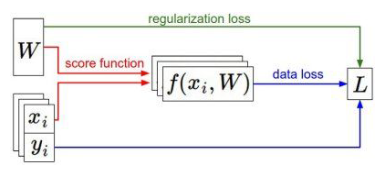
\includegraphics[width=0.42\textwidth]{pic/Lec3/Recap.png}
    \caption{Recap}
\end{figure}

\subsection{Optimization}
A way of efficiently finding the parameters that minimize the loss function.

Follow the slope. In 1-dimension, the derivative of a function:
\begin{align*}
    \frac{df(x)}{dx}=\lim_{h\rightarrow 0}\frac{f(x+h)-f(x)}{h}
\end{align*}
In multiple dimensions, the \textbf{gradient} is the vector of (partial derivatives) along each dimension. 

The slope in any direction is the \textbf{dot product} of the direction with the gradient.  The direction of steepest descent is the \textbf{negative gradient}. 

Use calculus to compute an analytic gradient $\nabla_W L$

\textbf{In summary}:
\begin{itemize}\small
    \item Numerical gradient: approximate, slow, easy to write
    \item Analytic gradient: exact, fast, error-pron
\end{itemize}

In practice: Always use analytic gradient, but check implementation with numerical gradient. This is called a \textbf{gradient check}.


\subsubsection{Gradient Descent}

\begin{figure}[!htb]
    \centering
    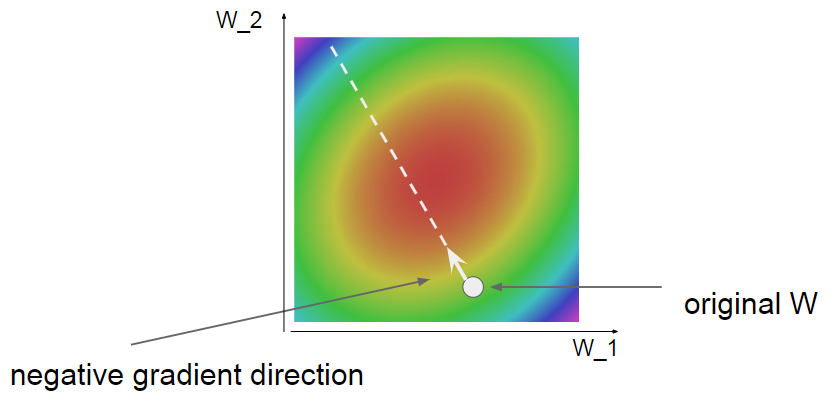
\includegraphics[width=0.42\textwidth]{pic/Lec3/Gradient Descent.png}
    \caption{Gradient Descent}
\end{figure}

走的步长是学习率属于超参数. 

\subsubsection{Stochastic Gradient Descent (SGD)}
Approximate sum using a minibatch


\subsection{Aside: Image Features}
\begin{figure}[!htb]
    \centering
    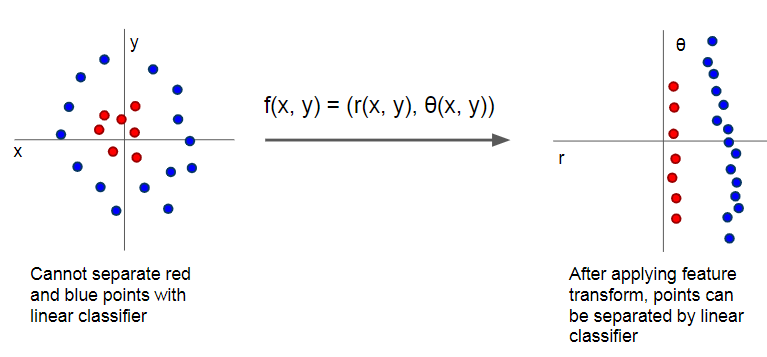
\includegraphics[width=0.42\textwidth]{pic/Lec3/Motivation}
    \caption{Image Features Motivation}
\end{figure}
有些时候不能直接分类, 把高维坐标下的点变换得易于分类

e.g. 
\begin{enumerate}
    \item Color Histogram
    \item Histogram of Oriented Gradients (HoG)
    \item Bag of Words
\end{enumerate}



